\subsection{Domain}
\label{sec:intro_domain}

This section outlines the theoretical background of each related knowledge domain involved in this research. The following list introduces each subsection:

\begin{itemize}
    \item Subsection \ref{sec:intro_fundamental_trading_strategies} describes the primary model which is a momentum strategy and why it was chosen.
    \item Subsection \ref{sec:intro_crypto_currencies} provides background about cryptoassets, cryptocurrencies and in particular Bitcoin and its ecosystem.
    \item Subsection \ref{sec:intro_financial_machine_learning} introduces the methodology Lopez de Prado explains in \cite{lopez_de_prado}, answers why machine learning is applied and introduces the structure break indexes with strong focus on SADF.
\end{itemize}

As detailed in \ref{sec:intro_problem_description}, the research problem involves many knowledge domains and data from different sources. When working in finance, models need to account for the independent variable time as markets \emph{evolve} with it, i.e. they are dynamic. Among all the available strategies to derive the primary model, momentum was chosen.

\subsubsection{Fundamental trading strategies}
\label{sec:intro_fundamental_trading_strategies}

There are many algorithmic fundamental trading strategies. We can use the classification in \cite{oxford_handbook}:

\begin{itemize}
    \item Impact driven: orders placed in a market affect the price of the stocks based on their volume and the liquidity. Strategies like volume-weighted average price (VWAP) or time-weighted average price (TWAP) can be found in this group.
    \item Cost driven: it not only considers implicit costs as the above but also the explicit costs of the market (e.g. commissions and access fees). We can find implementation shortfall in this group.
    \item Newsreader: based on the semi-strong form efficiency, these algorithms exploit news feeds to derive trading signals out of non-structured data.
    \item Market making: this group exploits the spread in the bid-ask prices.
    \item Statistical arbitrage: strategies in this group focus on two main premises: an asset tends to a \emph{medium} value in the long run (one can profit from deviations) or an asset's price is nonstationary, i.e. it fluctuates without a central value (one can profit from the tendency estimation). Mean reversion and momentum strategies belong to this group.
\end{itemize}

Momentum based strategies focus on deriving when a price starts to rise and drop to derive signals and profit by placing long and short positions on the asset. To derive these events, two different speed (fast and slow) moving average signals are used. The specific timestamps at which the fast and slow averaged signals cross determine an event. A fast signal crossing above the slow signal generates a buy event and the opposite generates a sell signal. A simple variation involves using exponential moving averages instead of simple moving averages and it increase complexity to even entire portfolios behind ETFs like MTUM (\cite{mtum_etf}).

In \cite{value_momentum} the authors explored the performance of momentum with market information of more than 200 years and confirm the strategy generally outperforms the market. In \cite{fact_fiction_momentum} the strategy is demystified in favor of a better comprehension of its strong and weak points. Based on the extensive literature around this strategy in particular, implementation simplicity, compatibility with the available data (no book order available, just stamped prices and volumes) this strategy was chosen to work as primary model.

\subsubsection{Cryptocurrencies}
\label{sec:intro_crypto_currencies}

Satoshi Nakamoto published \cite{bitcoin} with the intention to kick start a decentralized peer-to-peer cash system. However, it did not only do that but also gave birth to a new technology hype which is in continuous evolution and now is heading to mature the stack of services on top of the blockchain technology (\cite{deloitte}).

Let me present a few useful definitions:

\begin{itemize}
    \item Bitcoin: is the software that facilitates the transfer and custody of the bitcoin currency.
    \item bitcoin: a cryptocurrency.
    \item Blockchain: is a transaction database, in this case of the Bitcoin software. It keeps track of all debits and credits of bitcoin applying a very clever and sophisticated fashion (see  \cite{blockchain} for a comprehensive description). 
\end{itemize}

Bitcoin's blockchain technology provides several features:

\begin{itemize}
    \item It is publicly distributed. There are no secrete transactions.
    \item Serves as a historical record of \emph{all} transactions.
    \item It is immutable. Transactions will only be appended in the shape of new information blocks, but the \emph{verified} past cannot be changed.
    \item It is secure, i.e. each transaction is cryptographically verified to ensure valid funds. 
\end{itemize}

Transactions are verified via a \emph{Proof-of-Work} (PoW) algorithm which requires nowadays specialized hardware to process the cryptographic algorithm in a timely and competitive manner. Timely and competitive go hand in hand because the first \emph{miner} in claiming the block hash (result of the PoW) obtains a bitcoin reward provided by the Bitcoin software. The block hash is expensive to obtain but easy to verify what makes the acceptance of a new block a fast process for the entire network.

So far, we have introduced some of the technical characteristics of Bitcoin and supporting technologies. It is important to mention what this payment network provides to users. On one hand we have the privacy. Transactions happen from one wallet \cite{wallet} to another (cryptography comes in to properly describe how they work which is out of the scope of this document) and there is no direct nor easy way to know how is the owner of the wallet. Simply, there is information record about the owner of the wallet operation other than the transaction ledger (the blockchain itself). On the other hand, Bitcoin runs on the internet (using TCP \cite{bitcoin_network}) even on countries with network traffic control which sets the basis to trade worldwide without any regulation.

Another important aspect about bitcoin is the issuance model. Miners are paid every time they append a new block and receive a reward in bitcoins. The reward was initially set to 50 bitcoins and Bitcoin would adjust the mining complexity to get a new block every ten minutes on average. On a 210,000 blocks basis, the reward gets reduced to a half although the complexity keeps on adjusting to have the same throughput of one block every ten minutes. The total amount of bitcoins to be issued is 21 million and we can see in figure \ref{fig:issued_bitcoins} the amount of bitcoins issued by April 2020.

\begin{figure}[!htb]
    \centering
    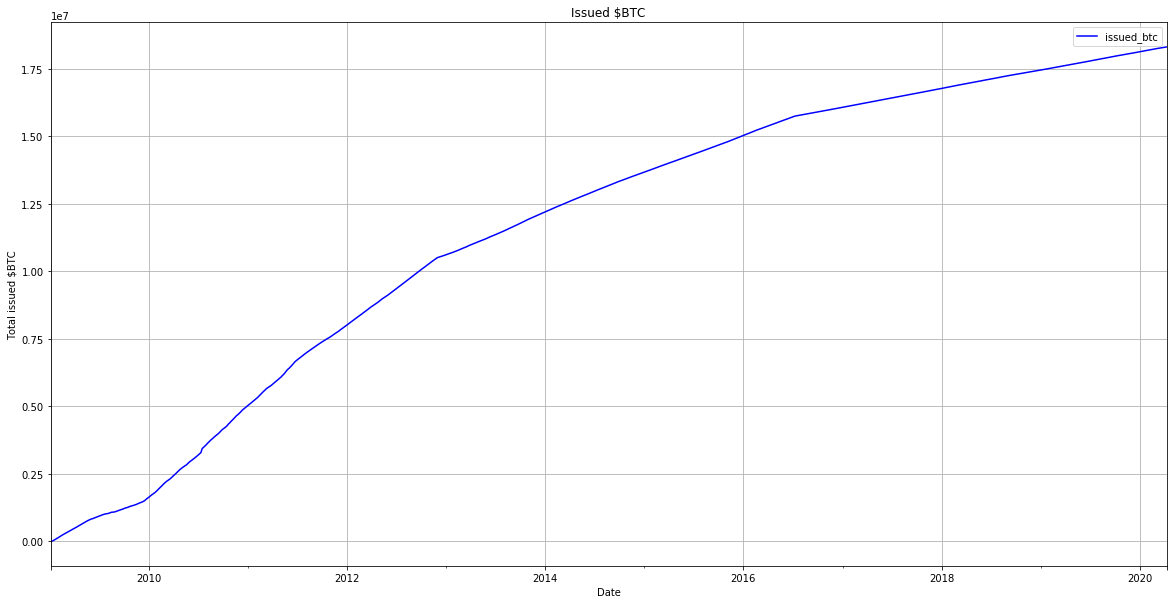
\includegraphics[width=\textwidth]{introduction/images/issued_btc.png}
    \caption{Issued bitcoins through time. Vertical scale is in tenths of millions of bitcoins. Glassnode data.}
    \label{fig:issued_bitcoins}
\end{figure}

And in \ref{fig:issuance} we can see the evolution of bitcoin issuance with time. By April 2021, the total amount of issued bitcoins is 18.66 millions roughly a 88.9\% of the 21 million.

\begin{figure}[!htb]
    \centering
    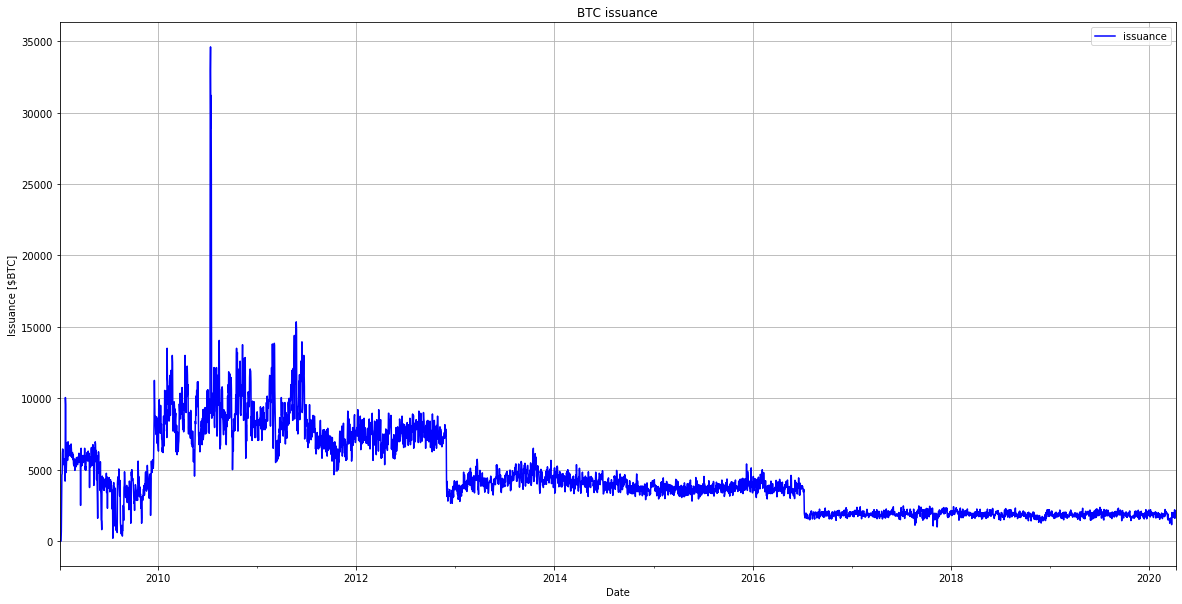
\includegraphics[width=\textwidth]{introduction/images/issuance.png}
    \caption{Bitcoin issuance through time. Glassnode data.}
    \label{fig:issuance}
\end{figure}

As it could be seen in \ref{fig:issuance} and in  \ref{fig:issued_bitcoins} the total number of bitcoins is decelerating. By design, bitcoin is a scarce asset. In \cite{bitcoin_stock_to_flow}, PlanB suggests to use a stock to flow (S/F) model to estimate the value of bitcoin scarcity. In figure \ref{fig:stock_to_flow} the close price series and the S/F ratio are shown to better explain its correlation. In blue we can see the how S/F ratio varies with time and in green we see the close price of bitcoin (note the vertical axis is plotted using a logarithmic scale). In red dotted vertical lines we see the days of the halvings (on 2012/11/28, 2016/07/09, and 2020/05/11). Along this feature (S/F ratio) others will be used that are very specific of the Bitcoin infrastructure and technology. Refer to \ref{sec:material_data_bitcoin_features} for a comprehensive description of the features.

\begin{figure}[!htb]
    \centering
    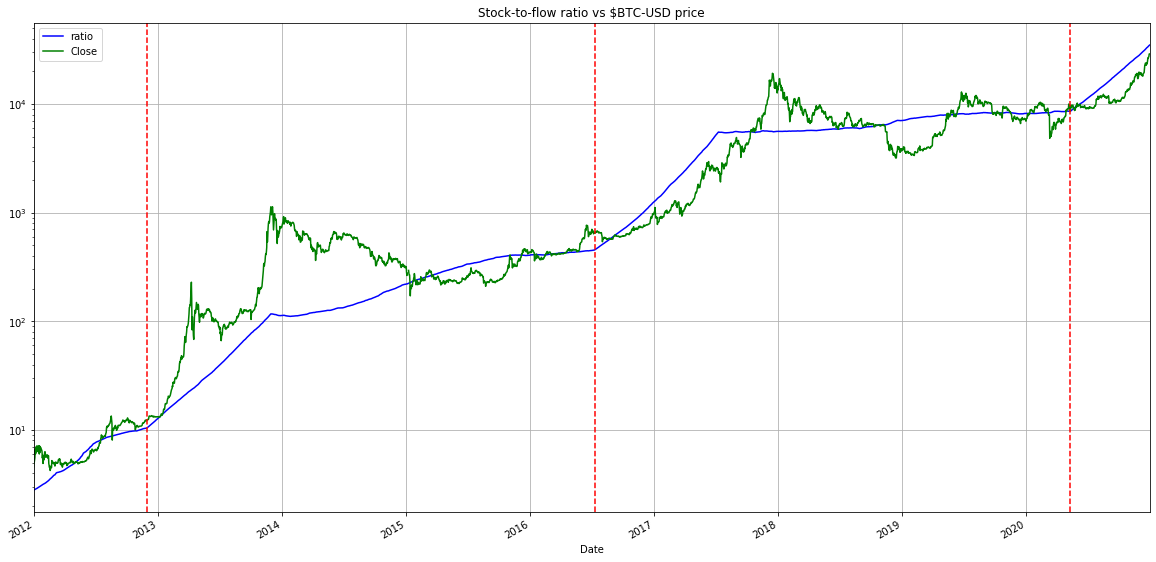
\includegraphics[width=\textwidth]{introduction/images/stock-to-flow.png}
    \caption{S/F ratio versus the close daily price in USD. Plotted in logarithmic vertical scale.}
    \label{fig:stock_to_flow}
\end{figure}

After Bitcoin software was released and gained attraction from different communities, other projects were created \emph{from} it (e.g. the so-called \emph{forks}). Bitcoin is an open source software project (\cite{bitcoin_github}) with a compatible license for both private and public usage which enabled people all around the world to use this technology for multiple purposes such as promotion of new bitcoin-like coins, projects running on top of the blockchain technology, etc.

In this research project we will use bitcoin: the top cryptocurrency by market capitalization as of April 2021 and the first cryptocurrency which started a revolution.

\subsubsection{Financial machine learning}
\label{sec:intro_financial_machine_learning}

This research project involves applied machine learning to finance where it is specifically applied to a trading strategy to learn the size of the position at each bet. In \cite{lopez_de_prado} it is described the procedure to properly develop a machine learning pipeline for a financial application like this one. Lopez de Prado described in \cite{future_of_empirical_finance} problems in financial research publications. The author relates those problems to bad practices and practitioners' ethics sometimes but he also recommended ways to mitigate those issues and their consequences. We could find a similar approach in \cite{lopez_de_prado} with a more in deep explanation of all the aspects which attain the machine learning pipeline to develop.  

As stated before, in this research project we will develop a strategy based on momentum to determine when and how (long vs. short) place our positions. That would define our primary model which follows a secondary model (the machine learning model) to derive the size of the position. Sizing the bet is a two step process: first  we obtain the probability that the buy or sell signal is accurate and second we compute the size of the the bet out of the probability. The model used to derive the probability could be a logistic regression, a tree based model, a neural network, a SVM or whatever model the researcher considers and \emph{finds} that yields better \emph{results}. This research project will focus on comparing some tree based models and evaluating based on \cite{lopez_de_prado} recommendations to mitigate common flaws that will certainly derive into runtime strategy biases and, consequently, losses.

In preparation to train the model, the well known feature engineering stage will be performed. In this case, univariate, bivariate, scaling and other techniques (\cite{feature_engineering}) are relevant but not enough. At least two chapters of \cite{lopez_de_prado} workout in detail two aspect of the time series analysis from a feature point of view: sample uniqueness (explained in section \ref{sec:methods_pipeline_secondary_model}) and sample stationarity (see chapter 15 \cite{time_series_analysis}) vs. loss of memory dilemma (explained in detail in section \ref{sec:methods_features}). One can find thorough explanations of the effects of bootstrap sampling and their effects on the model error (see section 7.11 of \cite{elements_of_statistical_learning}) but it does not usually consider the \emph{duration} of a sample because those in the dataset are often considered both independent and identically distributed (IID) as well as without duration. This is not the case of financial events like this one. Two or more \emph{signals} might overlap due to high volatility in the market or to correlated information. If the model does not take into account that those \emph{signals} refer to the same unique \emph{event} we would incur in unbalanced datasets when training a model due to variations in \emph{event} representativeness. On the other hand, to perform inference we require signals to be stationary but that comes at the expense of removing memory which is essential to obtain the predictive power. Lopez de Prado proposes to use fractional differentiation (see \cite{frac_diff_paper} for the possibly first known occurrence of the method) to determine the minimum differentiation factor $d$ such that the non stationarity null hypothesis of the series is rejected. Hence, some memory will remain in the series and the model can benefit from it.

\begin{figure}[!htb]
    \centering
    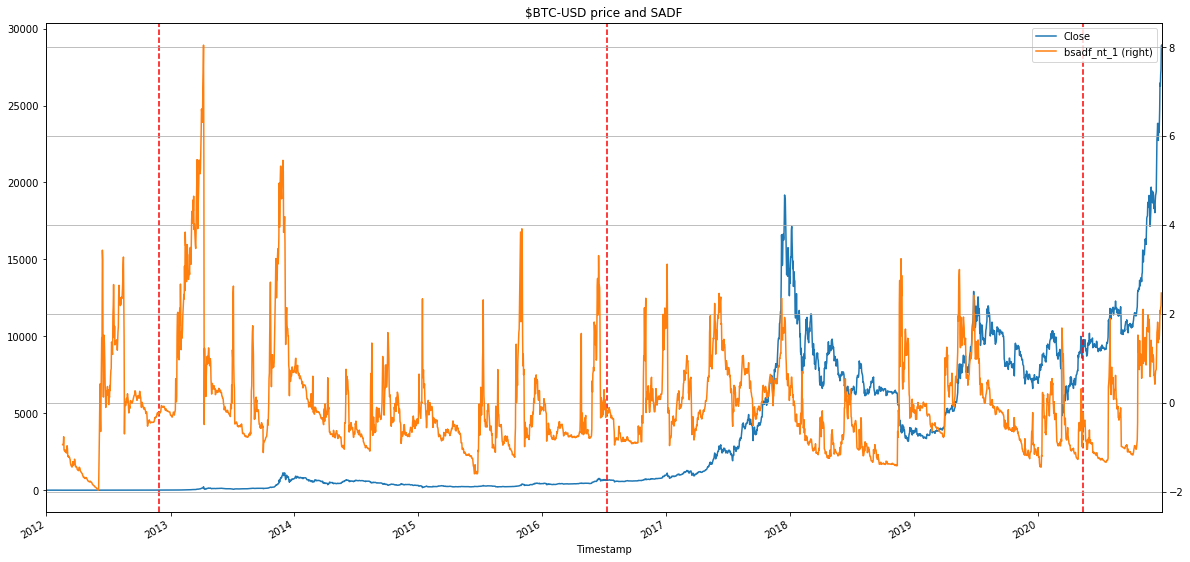
\includegraphics[width=\textwidth]{introduction/images/sadf_vs_price.png}
    \caption{Bitcoin price evolution and SADF index.}
    \label{fig:sadf_vs_price}
\end{figure}

\begin{figure}[!htb]
    \centering
    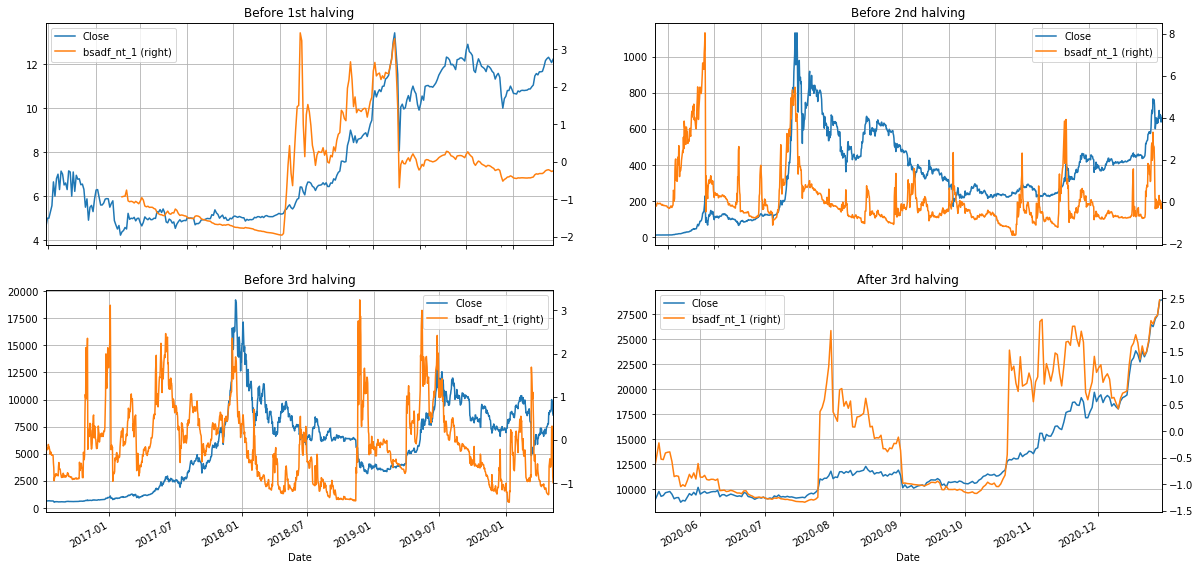
\includegraphics[width=\textwidth]{introduction/images/sadf_per_period.png}
    \caption{Bitcoin price evolution and SADF index by issuance period.}
    \label{fig:sadf_by_halving}
\end{figure}

In \ref{sec:intro_crypto_currencies}, the Stock to Flow model and halvings were introduced. The scarcity model and the issuance scheme imply regime breaks in the price series. Those events are called \emph{structural breaks} and specific features can be built to provide prediction power to our models, see \ref{sec:methods_features_sadf}. In chapter 17 of \cite{lopez_de_prado}, the author classifies into four the types of structural break tests: CUSUM tests, explosiveness tests, right-tail unit-root tests and sub/super-martingale tests. One can find within the explosiveness tests the Supremum Augmented Dickey-Fuller test (SADF, \cite{sadf_paper}) which evaluates successive bubble-like behaviors. The core idea of the index is that the price follows a random walk series and at some point it becomes an explosive test which ends up in a bubble burst. This process could repeat. The SADF index would raise when the bubble is growing and drastically decrease when the bubble explodes. Figure \ref{fig:sadf_vs_price} shows the evolution of the index over the prices. It is not trivial to see the relevance of this index unless we partition the price series by halvings and see it in figure \ref{fig:sadf_by_halving}.


Moreover, cross validation for training will be discussed and some tweaks we can use to improve the training technique as well as which model metrics we should use to compare machine learning models. Once all the features and the pipeline to train the model is in place, dimensionality reduction by feature selection will be applied to reduce the amount of required data while preserving model performance. Here, different methods will be compared in favor of increased decision robustness. Finally, backtesting of the strategy will be performed with strong emphasis on the the methodology.
